\chapter{相关工作}

\section{Web~服务相关技术}

\subsection{Web~服务与服务质量的基本概念}
Web服务是一种面向服务的架构技术,具体来说,Web~ 服务是一个平台独立的、松耦合的、自包含的、基于可编程的Web~应用程序,可以使用开放的XML 标准描述、发布、发现、协调和配置这些程序,用于开发分布式的互操作的应用程序。Web~服务是松耦合的软件模块,其之所以不同于以前的分布式计算体系结构,关键的一点在于,Web~服务协议、接口和注册服务可以使用松耦合的方式协同工作。为了做到这一点,服务接口的定义必须中立,独立于任何底层平台、操作系统以及实现服务所使用的编程语言。因此,服务可以在不同的系统上被实现,并以一直的形式以及通用的方式进行交互。Web~ 服务是一个完成单个任务的自包含的软件模块,该模块描述了自身的接口特征,基于这些信息,其他的服务能够确定该服务能完成什么功能,确定如何调用这些功能以及确定可能的结果。Web~ 服务提供了编程式访问,可将Web~ 服务嵌入到远程应用中,这个特性给Web~服务带来最大的附加值,换句话说,Web~ 服务的这个特性使得其可以和其他的软件模块或者应用程序集成,交换数据,完成更强大的功能。Web~服务的描述语言是基于XML 的,它既能描述Web~ 服务的功能性特征,又可以描述Web 服务的非功能性特征。Web服务使用的通信协议是基于http~ 的,因此非常通用,故而可以方便的在网络上分发Web~服务。

区分相同功能服务的一个重要标准是服务质量(Quality of Service,~QoS),其通常用来描述一个服务的非功能性属性。QoS之所以可以用来区分Web服务,是因为其可以作为衡量一个服务在执行时性能好坏的基准。常用的一些QoS~属性,例如:响应时间(Response time)、价格(Price)、可用性(Availability)、可靠性(Reliability)、吞吐率(Throughput)以及信誉度(Reputation)都可以作为评价这些服务性能的标准。它们都会被写进服务水平协议~\cite{andrieux2007web}~(Service Level Agreement,~SLA)作为服务定义的一部分~\cite{zeng2003quality}~。 简单来看一些这些属性的定义:

\begin{itemize}
  \item 响应时间:它是指服务的调用者从发出一个请求,到收到响应所经历的时间;
  \item 价格:它是指服务的调用者调用Web~ 服务所需要支付的费用;
  \item 可用性:它是指服务能正常执行的概率,数值越高代表Web~服务能够正常执行的可能性越大,反之,代表Web~服务出现异常的可能性越大;
  \item 可靠性:它是指服务能够正确地、始终如一地运行,并且无论系统或网络是否发生故障,都能提供同样的服务质量;
  \item 吞吐率:它是指服务在一个特定时间内所能处理的请求数;
  \item 信誉度:它是指Web~服务在功能属性和非公能属性的实际表现与发布该服务时所宣称状况的相符程度。
\end{itemize}

\subsection{Web~服务体系结构}

面向服务的体系结构(Service-Oriented Architecture,~SOA)是一种设计软件的逻辑方法,其通过发布标准接口,向网络上的其他服务提供服务。SOA 的主要目的就是使得已有的技术间具有通用的互操作性,并使得未来的应用和体系结构具有可扩展性。面向服务的体系结构中主要包含三个角色:服务提供者、服务调用者以及服务注册中心,SOA主要就是基于这三个角色进行交互。

\begin{itemize}
  \item 服务提供者:从企业角度看,服务提供者是服务的所有者;从体系结构的角度看,服务提供者是一个提供服务访问的平台;
  \item 服务调用者:从企业角度看,服务调用者是需要满足一定功能的企业;从体系结构角度看,服务调用者是搜索并发起执行服务的一个应用;
  \item 服务注册中心:服务注册中心是一个可供搜索的目录,服务提供者可以在这个目录中发布自己的服务,服务调用者可以在这个目录中搜索满足自己需求的服务。
\end{itemize}

这三个角色在交互的时候还会涉及到一些必要的操作,分别为:服务的发布、服务的查找、服务的绑定与调用。

\begin{itemize}
  \item 服务的发布操作:服务提供者利用Web 服务描述语言(Web Services Description Language,~WSDL)描述其需要发布的服务,主要需要描述Web服务的业务信息、服务信息、以及技术信息,然后将记录了这些信息的WSDL 文件发送到服务注册机构中,服务注册机构将这些信息存储到其数据库中,至此服务提供者完成了服务的发布,只有发布到服务注册机构的服务才有可能被服务调用者发现;
  \item 服务的查找操作:服务的查找操作通常会继续分为两个子操作,即服务的搜索以及服务的选择,具体来说,服务调用者去服务注册中心查找满足其需求的Web~ 服务,服务注册中心在接受到这个请求后,在后台数据库中搜索满足其需求的所有服务返回给调用者,然后调用者根据自身的情况,在这个结果集中选择一个最符合其要求的服务;
  \item 服务的绑定与调用操作:服务调用者在服务注册中心找到了符合自己要求的服务后,可以根据其描述文件中的服务地址来调用服务。
\end{itemize}

图~\ref{F:Fig_SOA}~展示了一个完整的Web服务体系结构,其包含了三个主要角色以及这些角色之间的交互操作。

\begin{figure}[thb]
    \centering
    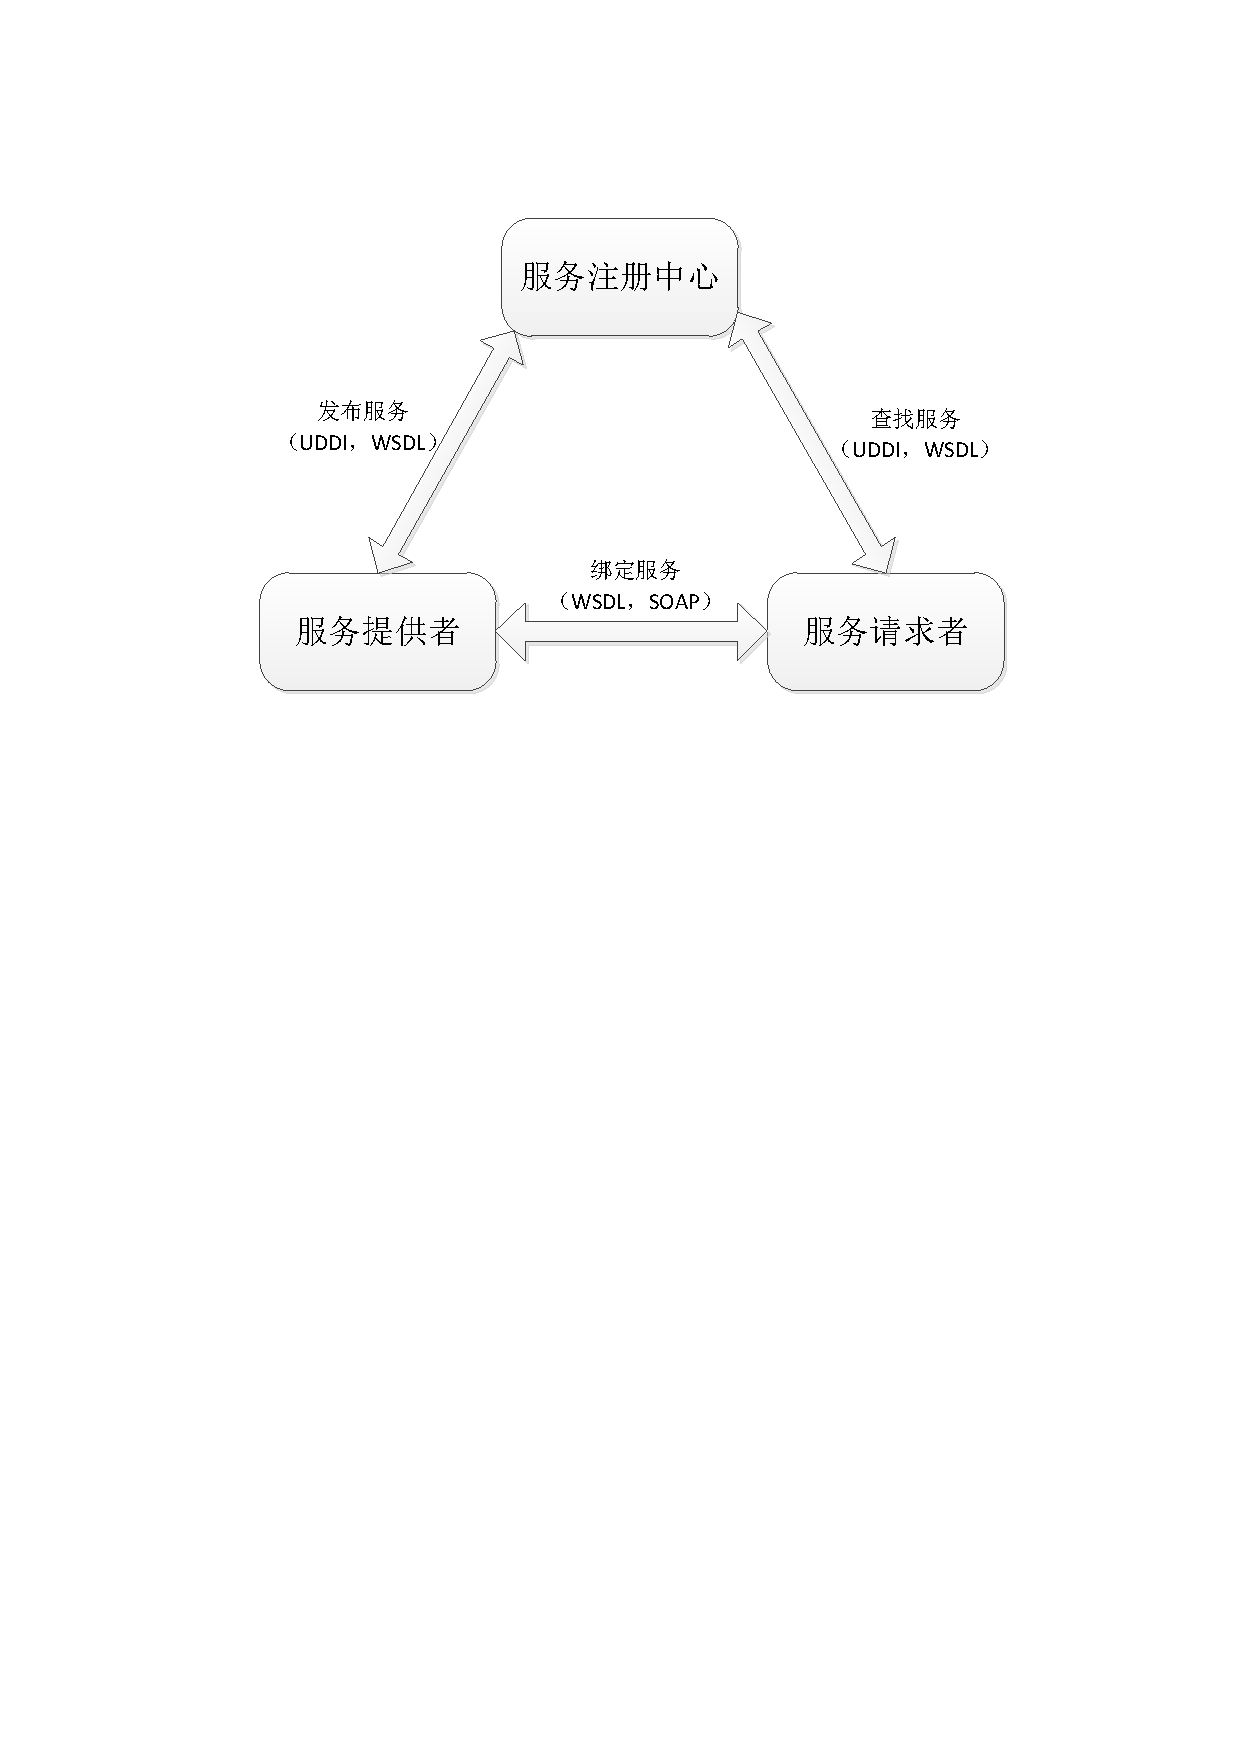
\includegraphics[width=0.6\textwidth]{./FIGs/Fig_SOA.pdf}
    \caption{SOA~体系架构}
    \label{F:Fig_SOA}
\end{figure}

\subsection{Web~服务技术基础}

Web服务技术由几类相关技术共同构成,一个被普遍认可的Web服务技术定义如图~\ref{F:Fig_WSTechArc}~ 所示~\cite{papazoglou2008web}~。

本节将会简要的介绍其核心部分,也就是图中的传输层、消息层、描述层以及发现层。
\begin{itemize}
  \item 传输层:Web~服务在传输层并没有限定采用何种传输协议,HTTP 是使用最为广泛的,因为HTTP的请求应答模式十分符合RPC类型调用,SMTP主要用于异步方式的调用,例如订阅信息等等;
  \item 消息层:消息层的协议定义了消息的格式,这一层是以SOAP为协议的。简单对象访问协议(Simple Object Access Protocol,~SOAP)是应用与分布式环境的,一种轻量级的、简单的、基于XML的协议,定义了封装机制和编码机制。SOAP 协议主要由四个部分组成:封装、编码规则、RPC表示以及绑定。封装定义了一个框架,该框架描述了消息中的内容是什么,谁应当处理它,以及它是可选的还是必须的。编码规则定义了一种序列化的机制,用于交换应用程序所定义的数据类型的实例。RPC 表示定义了用于表示远程过程调用和应答的协定。绑定定义了一种使用底层传输协议来完成在节点间交换SOAP 封装的约定。因为该协议与对象访问实质上没有关系,因此,在1.2版本之后,就成为了一个独立的词,而不再解释为Simple Object Access Protocol的缩写。
  \item 描述层:描述层的协议用于对如何使用这个Web~服务进行描述,描述信息一般包括使用到的数据类型、消息格式、方法名称和参数,该层主要使用Web~服务描述语言(Web Services Description Language,~WSDL)来描述一个服务。WSDL 由W3C指定,是一种基于XML 的接口定义语言,规定了如何描述Web~ 服务的功能,Web~服务的位置以及Web~服务的调用方式等。WSDL~ 规范中包括服务接口定义和服务的具体实现。服务接口定义描述了服务接口支持的操作,包括操作的类型、参数以及抽象数据类型。服务实现描述了服务部署的位置以及调用协议等。WSDL~元素主要包括以下几类:
      \begin{itemize}
        \item portType:Web~服务执行的操作,它可描述一个Web~服务可被执行的操作,以及相关的消息,可以把portType 元素比作传统编程语言中的一个函数库;
        \item message:Web~服务使用的消息,其定义一个操作的数据元素,每个消息均由一个或多个部件组成,可以把这些部件比作传统编程语言中一个函数调用的参数;
        \item types:Web~服务使用的数据类型,其定义Web~服务使用的数据类型,为了最大程度的平台中立性,WSDL使用XML Schema语法来定义数据类型;
        \item binding:Web~服务使用的通信协议,其为每个端口定义消息格式和协议细节。
      \end{itemize}
  \item 发现层:使用UDDI(Universal Description, Discovery and Integration,通用描述、发现与集成服务)可进行Web~ 服务的发布。UDDI 是一个公开目录,可提供在线服务的发布,并有助于Web~ 服务的最终发现。公司可以发布它们所提供的服务的WSDL规范, 其他公司根据这个WSDL 描述来访问那些服务。
\end{itemize}

\begin{figure}[thb]
    \centering
    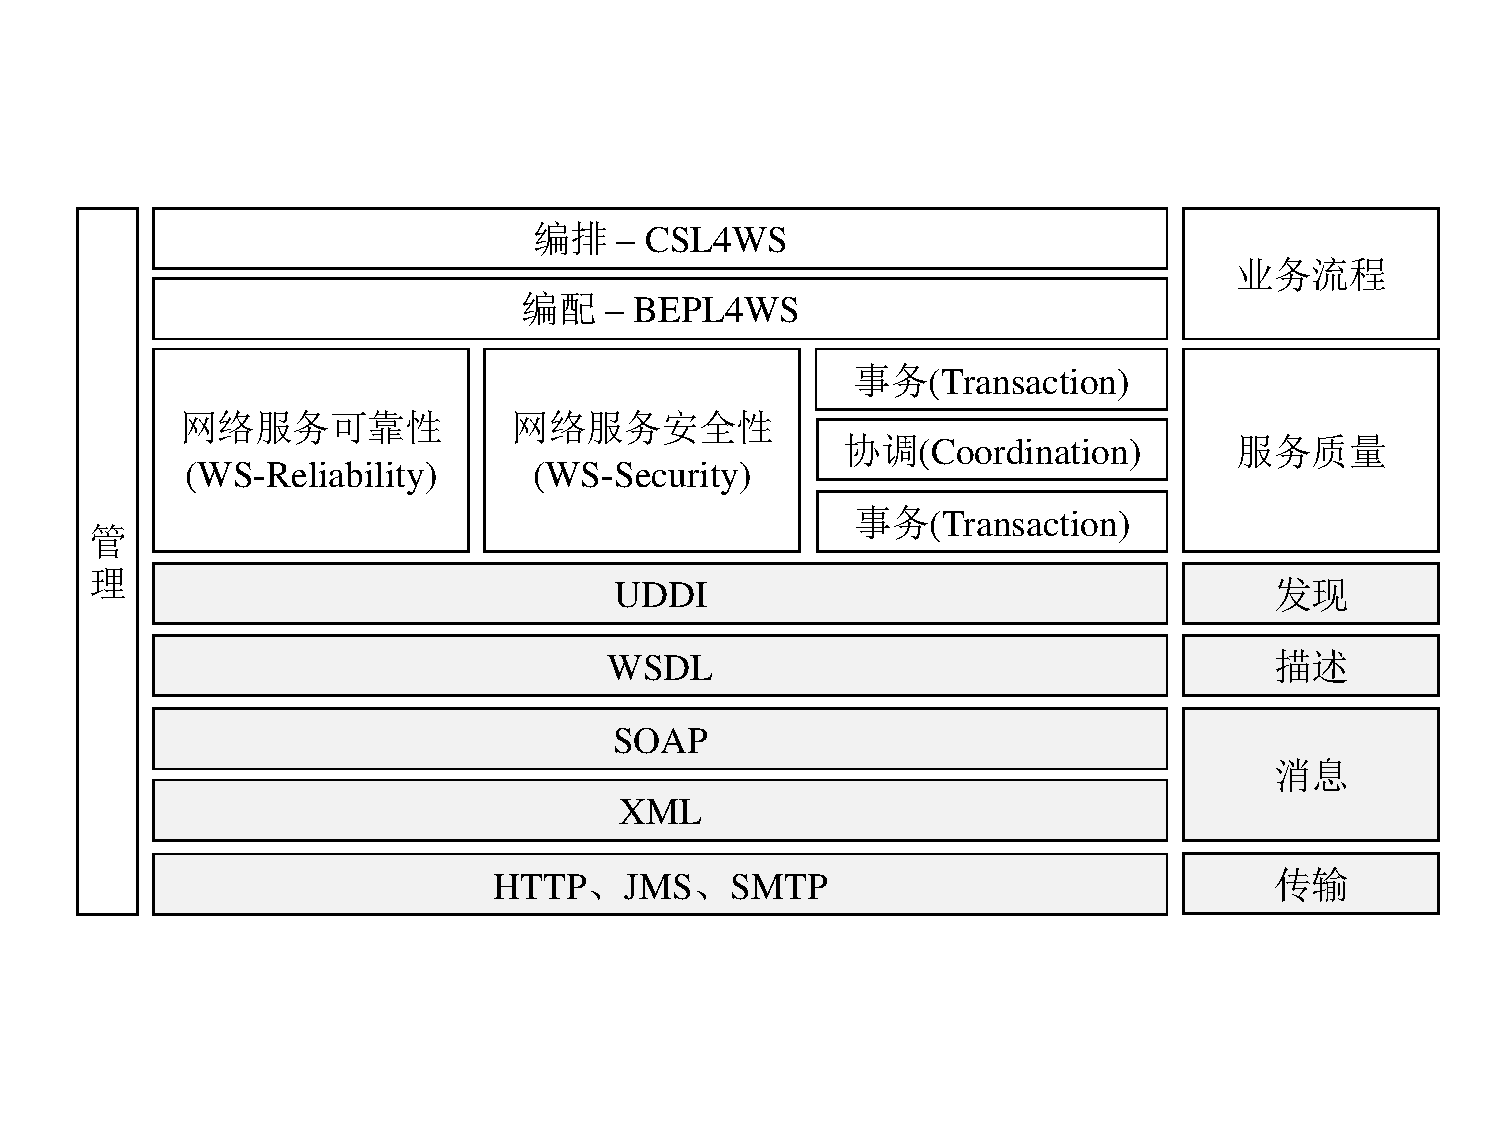
\includegraphics[width=0.9\textwidth]{./FIGs/Fig_WSTechArc.pdf}
    \caption{Web~服务技术架构}
    \label{F:Fig_WSTechArc}
\end{figure}


\section{Web~服务组合相关概念}

Web~服务技术为异构、自治和松耦合的分布式应用提供了一个集成和交互的机制。但是单一Web~ 服务的功能毕竟有限,难以满足某些实际应用的需求,因此有必要对这些单一的Web~服务进行合成,从而生成功能更加复杂、更加强大的组合Web 服务来满足这些实际应用的需求,随着Web~ 服务应用的不断深入,Web~组合技术也得到了工业界和学术界的广泛关注。

为使得表述方便,本文约定几个关于服务的概念:

\begin{definition}[原子服务]
    原子服务是指可独立完成一个功能的具体服务,且不可以再被拆分,记为$s$。
\end{definition}

\begin{definition}[服务质量QoS]
    服务质量由若干服务质量属性组成,记为$\emph{Q}=\{q_{1},\ q_{2}, \cdots, q_{d}\}$,一个原子服务的\emph{QoS}值为$\emph{QV}(s)=\{q_{1}(s),\ q_{2}(s), \cdots, q_{d}(s)\}$。
\end{definition}

\begin{definition}[抽象服务]
    抽象服务是对一类提供相同功能的原子服务的抽象,一个原子服务一定是一个抽象服务的实例记为$S$。
\end{definition}

\begin{definition}[候选服务集合]
    每一个抽象服务都对应一个候选服务集合,候选服务集合由一组提供与抽象服务相同的功能的原子服务构成,记为$\emph{CndS}=\{s_{1},\ s_{2},\ \cdots,\ s_{n}\}$。
\end{definition}

\begin{definition}[抽象组合服务]
    抽象组合服务由一组抽象服务组合而成,用以实现更加复杂的功能,记为$\emph{ACS}=\{S_{1},\ S_{2},\ \cdots,\ S_{m}\}$。
\end{definition}

\begin{definition}[组合服务]
    组合服务是抽象组合服务的一个实例。通过为抽象组合服务中每一个抽象服务绑定一个原子服务,来得到一个组合服务,记为$CS$。
\end{definition}

基于QoS的Web~服务选择问题是,在确定了一个抽象组合服务后,如何从每一个抽象服务的候选服务集合中,分别挑出一个原子服务绑定到抽象服务上,使得最终得到的组合服务在满足用户约束的条件下,组合服务的整体QoS 最高。

一个组合服务的QoS值是由构成它的原子服务的QoS聚合而成,聚合函数~\cite{alrifai2012hybrid}~如表~\ref{T:Tab_QoSAgg}~所示:


%表格:聚合函数

%p参数本身就指定了一个列,后面加个lcr只能再起新的一列
%比较方便的方法是使用array宏包\usepackage{array}
%如下代码即可实现文字居中
%\begin{tabular}{|p{2cm}<{\centering}|}
%居中
%\end{tabular}

%&\tabincell{c}{something\\ %一个单元格内换行
%something}
\begin{table}[!thp]
\centering  % 表居中
\renewcommand{\arraystretch}{1.1} %设置表格间距
\begin{tabular}{|p{5cm}<{\centering}|p{5cm}<{\centering}|}  % {} 表示各列元素对齐方式,left-l,right-r,center-c
\hline
QoS属性 & 聚合函数 \\\hline\hline
%响应时间
Response Time & $\sum^{j=1}_{n}q(s_{j})$ \\\hline
%价格
Price & $\sum^{j=1}_{n}q(s_{j})$ \\\hline
%可用性
Availability & $\prod^{j=1}_{n}q(s_{j})$ \\\hline
%可靠性
Reliability & $\prod^{j=1}_{n}q(s_{j})$ \\\hline
%吞吐量
Throughput & $min^{j=1}_{n}q(s_{j})$\\\hline
%信誉度
Reputation & $\frac{1}{n}\sum^{j=1}_{n}q(s_{j})$ \\\hline
\end{tabular}
\caption{QoS聚合函数}\label{T:Tab_QoSAgg}
%\vspace{5pt}
\end{table}
%表格结束:服务集合

表中的聚合公式适用于抽象组合服务为顺序结构的情况,本文的研究主要是基于顺序结构的抽象服务进行的。如果考虑其他抽象服务的结构,例如选择、循环等,QoS聚合函数将更加服务杂,不过在文献~\cite{cardoso2004quality}~ 中,作者提出了一种方法将组合服务中的选择、循环等结构转换为顺序结构,然后再利用表~\ref{T:Tab_QoSAgg}~中的聚合函数计算组合服务的QoS 值。

由于一个原子服务的QoS通常有多个属性,每种QoS属性的单位以及其值所在的范围域都可能不同,因此不利于不同QoS属性间的评估或比较,为了解决这个问题,有学者提出了效应函数(Utility function)的概念,它通过比较候选服务集合中所有的原子服务,将原子服务的QoS属性值映射到到一个实数值,并通过该值来描述相应的QoS属性,通过这种映射,不同的QoS属性就可以在同一的标准下进行计算和评估。公式~\ref{E:EQ_UtiliySum}~ 给出了候选服务QoS属性的效应函数~\cite{alrifai2012hybrid}~。

\begin{align}
& U(s_{ij})=\sum^{d}_{k=1}\frac{Q_{max}(i,k)-q_{k}(s)}{Q_{max}(i,k)-Q_{min}(i,k)}  \label{E:EQ_UtiliySum} \\
& Q_{max}(i,k)=\mathop{max}_{\forall s_{ij} \in S_{i}}(q_{k}(s_{ij}))  \label{E:EQ_UtiliyMax} \\
& Q_{min}(i,k)=\mathop{min}_{\forall s_{ij} \in S_{i}}(q_{k}(s_{ij}))  \label{E:EQ_UtilityMin}
\end{align}


\begin{definition}[归一化]
利用效应函数对候选服务集合中原子服务的\emph{QoS} 进行映射的过程,我们称之为归一化。
\end{definition}

关于主流的Web服务组合方法以及Web服务选择策略已在~\ref{S:SEC_StateOfArt}~节讨论过,故而这里不再对此部分进行赘述。前文已经提到,基于Skyline 的混合策略可以大大缩减服务选择的范围,因而近年来在服务选择领域,越来越多的学者也开始关注如何利用Skyline~中的技术来解决服务选择问题。下一节将对Skyline~的相关概念进行介绍。

\section{Skyline~相关概念}

\subsection{Skyline~计算介绍}

Skyline计算就是从一个数据库中不断的计算不被数据库中其它任何数据对象支配的数据对象,最终得到一个数据对象集合。Skyline 查询经常被用来解决多目标决策问题。

\begin{definition}[支配]
    我们称数据对象$p_{i}$支配(dominance)数据对象$p_{j}$,当且仅当$p_{i}$ 的每个属性都和$p_{j}$的一样好,且在$p_{i}$ 中一定有一个属性比$p_{j}$的要好,记为$p_{i} \succ p_{j}$。
\end{definition}

图~\ref{F:Fig_SkylineHotel}~是一个经常用来解释Skyline计算的例子:假设有一个人在假期的时候想去一个景区玩,景区周围有很多宾馆,在上图坐标系中的一个个点就代表着一个个宾馆,坐标系的横坐标代表着某宾馆距离景区的距离,纵坐标代表着宾馆的价格。对于游客来说,他想找到的是距离景区近,且价格便宜的宾馆,他要从这么多宾馆中去选择效率一定很低。然而我们发现游客只需要从\emph{宾馆a}、\emph{宾馆i}、\emph{宾馆k} 中去挑选即可,这是因为坐标系中的其他宾馆在价格与距离上面都不如这三个宾馆好,且这三个宾馆两两之间都无法在两个维度上都比对方更好。换句话说,这三个宾馆互相不支配,且坐标系中的其他宾馆都被这三个宾馆中的某个或多个支配。这三个宾馆构成的集合就是Skyline。 确定这三个宾馆的过程,就是Skyline查询。在这个例子中,一个属性比另一个好,体现为数学关系上的``\emph{小于}''。为了简单起见,在本文的后续部分,如果不加特殊说明,我们都假定一个属性的值越小,那么其属性越好。

\begin{figure}[thb]
    \centering
    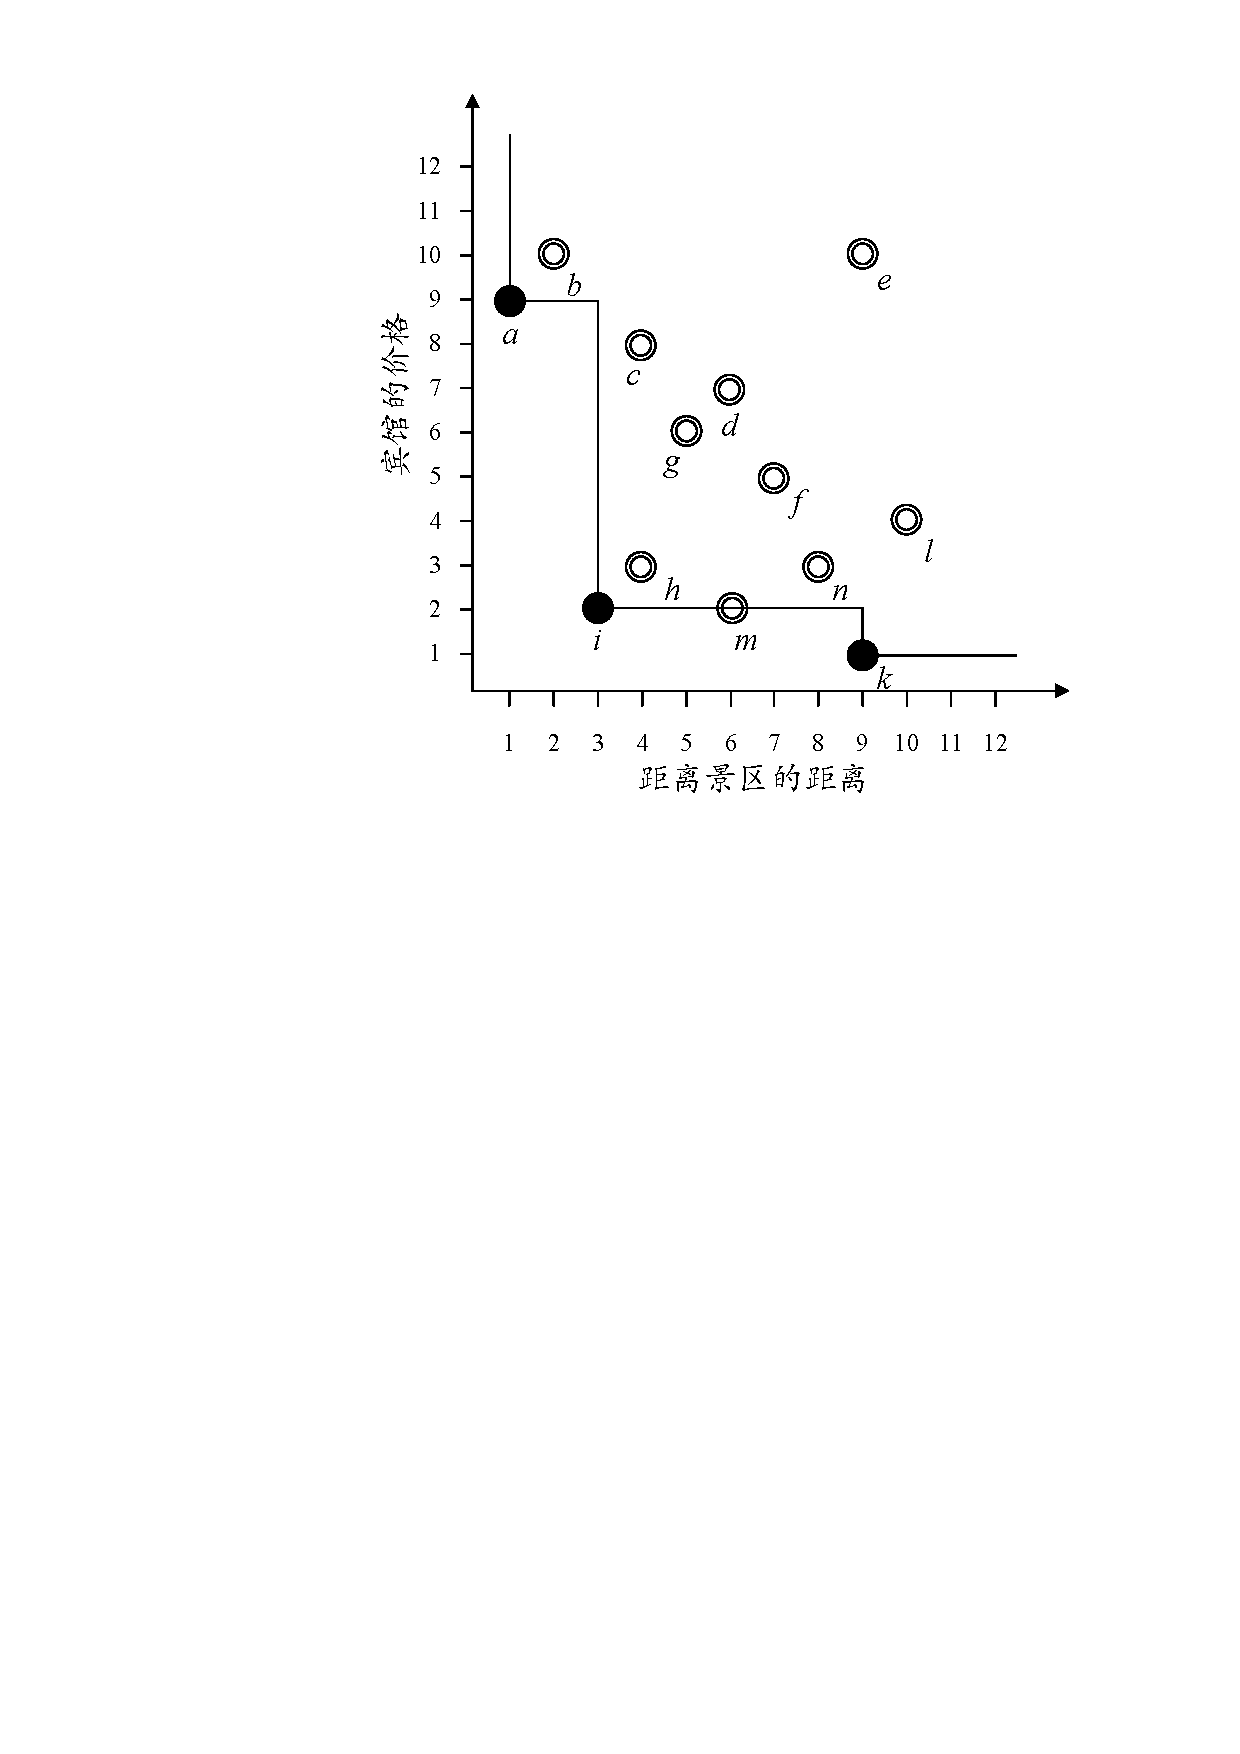
\includegraphics[width=0.6\textwidth]{./FIGs/Fig_SkylineHotel.pdf}
    \caption{Skyline计算的例子}
    \label{F:Fig_SkylineHotel}
\end{figure}

\subsection{Skyline~计算算法介绍}

Skyline计算已经在数据库领域被广泛关注~\cite{yu2013efficient}~,分治算法(divide-and-conquer,~D$\&$C)~\cite{borzsony2001skyline}~以及块嵌套环算法(block nested loop, BNL)~\cite{borzsony2001skyline}~是最早被设计用来处理Skyline 计算问题的。基于BNL算法,在文献~\cite{chomicki2003skyline}~中,作者提出了排序过滤算法(\emph{sort filter skyline}, SFS),它在计算Skyline前先对候选服务进行排序,通过该预处理操作提高计算的效率。LESS算法(linear elimination sort for skyline, LESS)~\cite{godfrey2005maximal}~对于SFS算法进一步改进,该算法在SFS预处理阶段移除一些不可能是Skyline的数据对象。位图算法(bitmap)~\cite{tan2001efficient}~利用了位操作,可快速计算出Skyline数据对象。索引算法(index)~\cite{tan2001efficient}~根据每一个数据对象中维度值最小的维度建立索引,然后分批计算出Skyline数据对象。最近邻算法(nearest neighbor, NN)~\cite{kossmann2002shooting}~基于Rtree 对数据集中的数据建立索引结构,利用数据对象距离远点的距离(用户可自定义距离函数),每一次选择距离原点最近的数据对象,该数据对象已经是Skyline,然后以此数据对象为中心,将数据空间继续划分成若干部分,在每一个部分上递归的运行,知道每个子部分只含有一个点为止。分支限定算法(\emph{branch and bound skyline}, BBS)~\cite{papadias2005progressive}~也是基于Rtree来做,与NN不同的是,BBS是通过遍历Rtree中的每一个节点(文中称其为MBR,Minimum Bounding Rectangle),通过比较不同MBR中距离原点最近的顶点来快速得到Skyline,相对于NN 来说,BBS 更简单。

\begin{enumerate}
  \item D$\&$C算法

  \begin{figure}[thb]
    \centering
    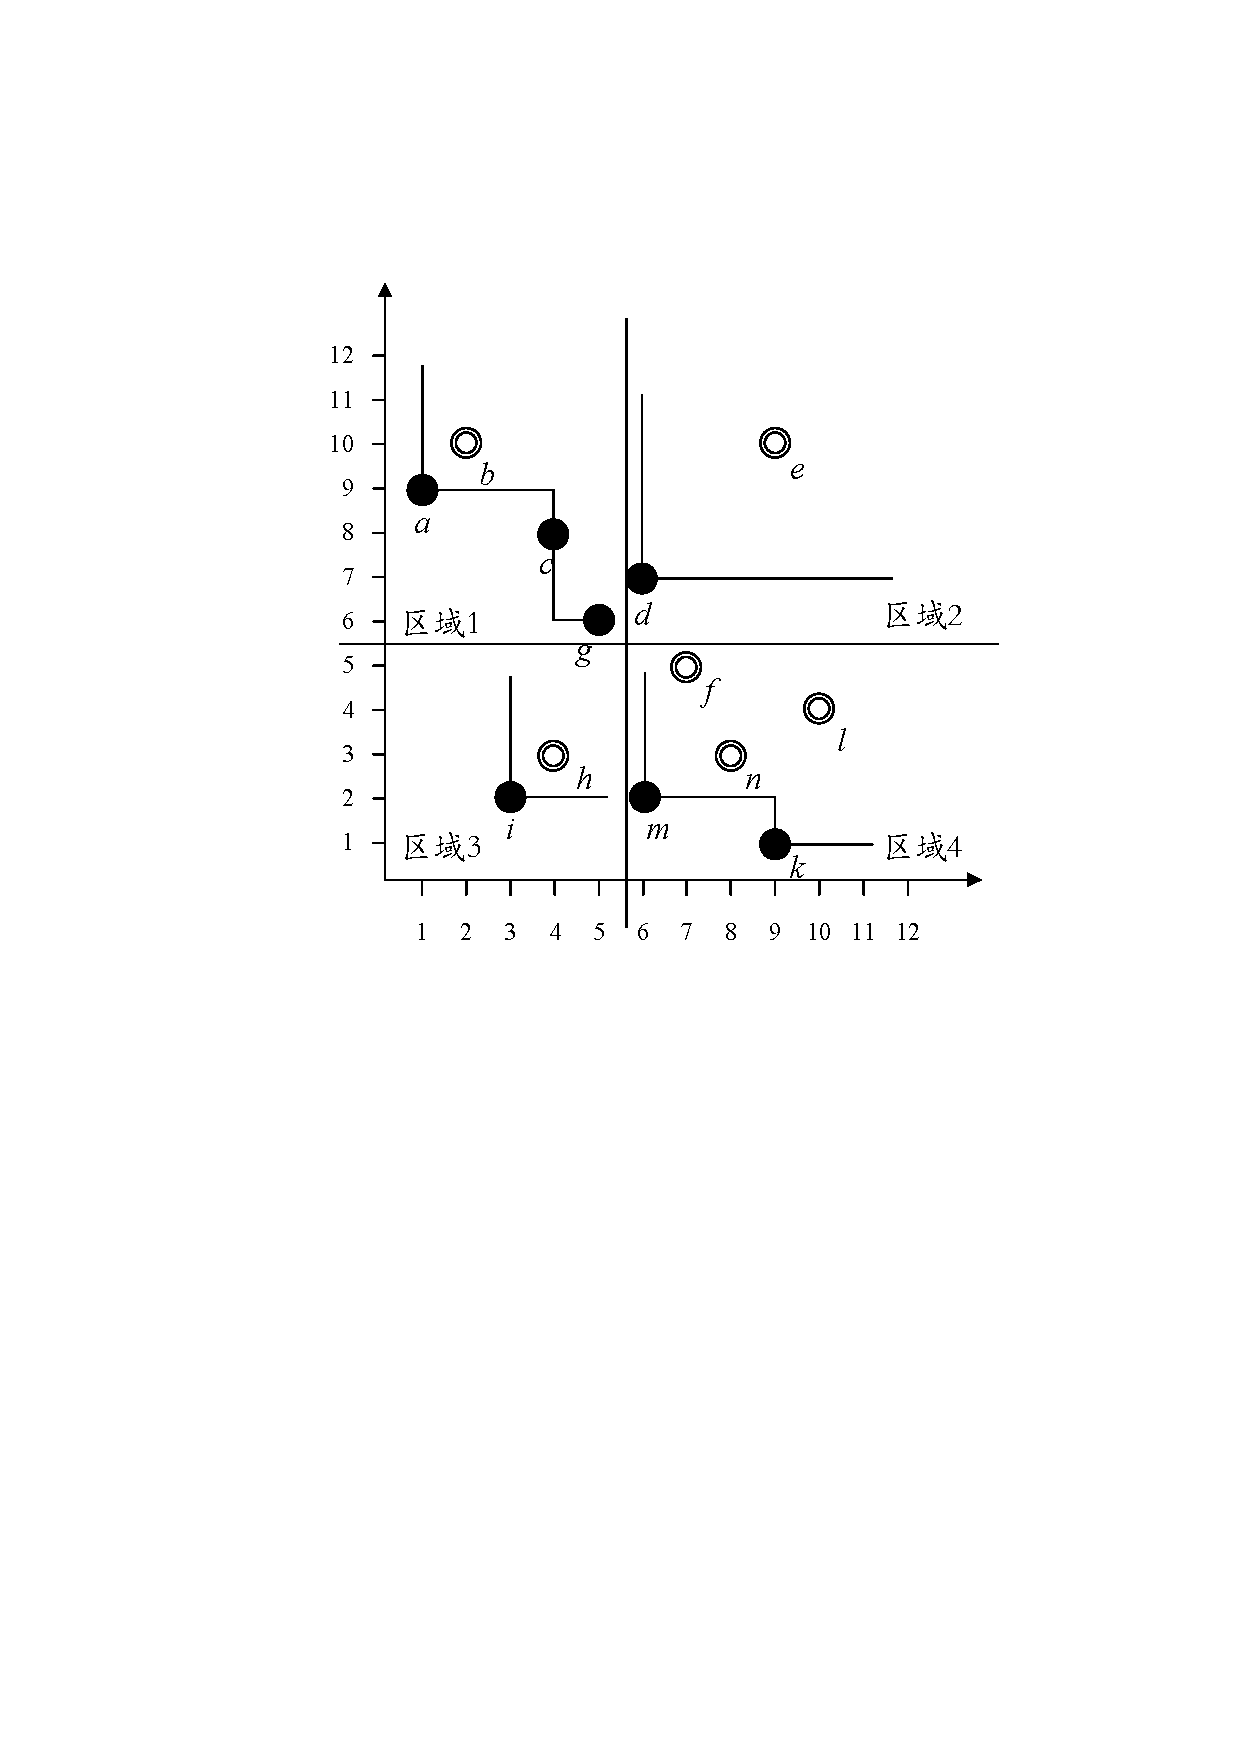
\includegraphics[width=0.6\textwidth]{./FIGs/Fig_SkyAlgoDC.pdf}
    \caption{D$\&$C算法例子}
    \label{F:Fig_SkyAlgoDC}
  \end{figure}

  D$\&$C算法将数据库中的数据划分成若干部分,使得每个部分都可以放入内存中。然后在每一个子部分中计算出Skyline数据对象,最终的Skyline 数据点通过合并计算每个子部分中的结果得到。如图~\ref{F:Fig_SkyAlgoDC}~所示,我们对图~\ref{F:Fig_SkylineHotel}~中的数据进行划分,划分成四个区域,分别包含\{$a$, $c$, $g$\},\{$d$\},\{$i$\}以及\{$m$, $k$\}。 为了得到最终的Skyline,我们需要移一些除被其他区域中数据对象所支配的数据对象。在区域2 中的数据对象显然需要被移除,因为它们都会被区域3 中的点移除,除非区域3为空。区域1中的数据对象只需要与区域3中的比较,这是因为区域2和区域4 中的数据对象都不可能支配区域1 中的数据对象。在本例中,数据$c$ 和$g$由于被$i$支配,所以被移除。同样的,区域4也只需与区域3比较即可,$m$被移除。最后,我们得到Skyline数据对象集合$\{a, i, k\}$。在数据集不是很大的时候u,D$\&$C算法有着很好的效率,但是对于较大的数据集(内存中不可一次载入),分割的过程会导致整个数据集被多次读写,从而导致磁盘I/O开销变得很大。除此之外,D$\&$C算法只能在所有的区域都合并后才能得到结果,不能在计算的同时就输出结果。

  \item BNL算法以及SFS算法

  最容易想到的Skyline计算方法就是将数据对象$p$ 与集合中的其他数据对象一一比较,如果集合中没有数据对象可以支配$p$,那么就将$p$ 作为Skyline输出。BNL算法就是受这种方法的启发,它在内存中维护着一个存放Skyline数据对象的链表,最初始的时候,里面存放着第一个数据对象,与此同时,对于后续的数据对象$p$,当$p$与链表内数据对象比较时候,有三种可能的情况:(\romannumeral1)如果$p$被链表中的某个数据对象支配了,那么它就会被丢弃,因为它不可能是Skyline的一部分;(\romannumeral2)如果$p$支配了链表中的某个数据对象,那么$p$将被插入,并且链表内所有被$p$支配的数据对象都将被丢弃;(\romannumeral3)如果$p$即不被别的数据对象支配,也没有支配其他数据对象,那么直接将$p$插入。

  这个链表是自管理的,所谓的自管理指的是,当链表中的某个数据对象被发现支配其他服务的时候,这个数据对象就会被移至链表首部。一般认为,如果一个数据对象支配了多个其他数据对象,那么它就可以支配更多的数据对象。BNL最大的问题在于,在算法运行的过程中,链表过大,导致其超出内存,此时,对于情况(\romannumeral3)中的数据对象,我们将其放在一个临时链表中。由于这个原因,BNL 算法可能需要被执行多次。在算法遍历完一遍所有的数据后,只有那些在临时链表创建前就存在于链表中的数据对象是Skyline数据对象。对于临时链表中的数据对象,需要应用BNL再次进行计算。

  BNL的优势在于其可以广泛的适应性,其可以在没有索引,没有排序的任何维度数据上直接应用。BNL的劣势在于,其对内存的依赖过高,如果内存过小,无疑需要BNL进行多次迭代计算,并在它也需要等到所有的数据遍历一遍才能输出第一个Skyline数据对象。

  SFS算法对BNL进行了改进,它先讲数据集中的所有数据对象进行排序,排序的依据是用户指定的一个单调函数。候选数据对象按照其分值从小到大顺序依次插入链表中,之所以这样做是因为,分值越小的数据对象越有可能支配更多的数据对象。从而进一步优化了剪枝的步骤。但是SFS输出Skyline点的顺序是固定的,不可以根据用户的偏好输出。

  \item Bitmap算法

    \begin{table}[!thp]
    \centering  % 表居中
    \renewcommand{\arraystretch}{1.1} %设置表格间距
    \begin{tabular}{|c|c|c|}
    \hline
    编号 & 坐标 & 位图表示 \\\hline
    $a$ & $(1, 9)$ & $(111111\textbf{1}111, 11\textbf{0}0000000)$ \\\hline
    $b$ & $(2, 10)$ & $(111111\textbf{1}110, 10\textbf{0}0000000)$ \\\hline
    $c$ & $(4, 8)$ & $(111111\textbf{1}000, 11\textbf{1}0000000)$ \\\hline
    $d$ & $(6, 7)$ & $(111110\textbf{0}000, 11\textbf{1}1000000)$ \\\hline
    $e$ & $(9, 10)$ & $(110000\textbf{0}000, 10\textbf{0}0000000)$ \\\hline
    $f$ & $(7, 5)$ & $(111100\textbf{0}000, 11\textbf{1}1110000)$ \\\hline
    $g$ & $(5, 6)$ & $(111111\textbf{0}000, 11\textbf{1}1100000)$ \\\hline
    $h$ & $(4, 3)$ & $(111111\textbf{1}000, 11\textbf{1}1111100)$ \\\hline
    $i$ & $(3, 2)$ & $(111111\textbf{1}100, 11\textbf{1}1111110)$ \\\hline
    $k$ & $(9, 1)$ & $(110000\textbf{0}000, 11\textbf{1}1111111)$ \\\hline
    $l$ & $(10, 4)$ & $(100000\textbf{0}000, 11\textbf{1}1111000)$ \\\hline
    $m$ & $(6, 2)$ & $(111110\textbf{0}000, 11\textbf{1}11111110)$ \\\hline
    $n$ & $(8, 3)$ & $(111000\textbf{0}000, 11\textbf{1}1111100)$ \\\hline
    \end{tabular}
    \caption{位图算法}\label{T:Tab_Bitmap}
    \end{table}

  顾名思义,位图算法是基于位图来计算数据对象之间的支配关系的。一个数据对象$p=(p_{1}, p_{2}, \cdots, p_{d})$可以被映射到一个$m$的向量中。假设$p$ 的第$i$维度属性值中一共有$k_{i}$个不同的值,那么这一个维度就可以用$k_{i}$个位来表说,从而对于$p$,一共需要$\sum_{i=1}^{d}k_{i}$个位来表示。在图~\ref{F:Fig_SkylineHotel}~ 中,$k_{1}=k_{2}=10$,故而对于其中的每一个点都需要20 位来表示。假设$p_{i}$属性的属性值是在$i$属性所有可能的值中第$j_{i}$小的,那么表示该属性的$k_{i}$位比特中,最左边的$(k_{i}-j_{i}+1)$位为1,剩下的部分为0。图~\ref{F:Fig_SkylineHotel}~的数据对象表示成位图如表~\ref{T:Tab_Bitmap}~所示。假设我们现在要确定$c$是否是Skyline,我们需要按照如下步骤计算:第一步分别在$c$ 的用位图表示的维度值中从左向右找到第一个1 所在的位置,得到的结果是4和8。然后我们将所有数据对象响应维度位图中的相应位的值取出(表格中的黑体表示),第一维度$c_{X}=1110000110000$,第二维度$c_{Y}=0011011111111$。接下来我们对这两个维度的位图做与操作得到$c_{X} \& c_{Y}=0010000110000$,意味着除了$c$自身之外,还有$h$与$i$支配它,因为它不属于Skyline。 位图算法的速度依赖于位操作的速度,但是如果需要确定一个点是否属于Skyline,必须要将该点与数据集内所有的点比较。

  \item Index算法

    %\leqslant和\geqslant
  索引算法将$d$维的数据对象分别分配到$d$个列表中,分配的依据是:如果一个数据对象$p={p_{1},p_{2}, \cdots, p_{d}}$被分配到第$i$列($1\leqslant i\leqslant d$),那么$p$ 的第$i$个维度的属性值一定是其所有属性值中之最小的那一个。表~\ref{T:Tab_Index}~中将图~\ref{F:Fig_SkylineHotel}~中的点映射到两个列表中。每一个列表中的数据对象会依据其最小维度的值进行排序,并且利用B- 树建立索引。具有相同的属性值的数据对象会被放置在同批次(batch)中,如列表2 中的$\{i,m\}$ 以及$\{h,n\}$。

  \begin{table}[t]
    \centering  % 表居中
    %\renewcommand{\arraystretch}{1.1} %设置表格间距
    \begin{tabular}{|c|c|c|c|}
    \hline
    \multicolumn{2}{|c|}{\tabincell{c}{List1 \\ 第1维度值比较小}} & \multicolumn{2}{|c|}{\tabincell{c}{List2 \\ 第2 维度值比较小}}  \\\hline\hline
    $a$ (1, 9) & $minC =$ 1 & $k$ (9, 1) & $minC =$ 1 \\\hline
    $b$ (2, 10)& $minC =$ 2 & $i$ (3, 2), $m$ (6, 2) & $minC =$ 2 \\\hline
    $c$ (4, 8) & $minC =$ 4 & $h$ (4, 3), $n$ (8, 3) & $minC =$ 3 \\\hline
    $g$ (5, 6) & $minC =$ 5 & $l$ (10, 4) & $minC =$ 4 \\\hline
    $d$ (6, 7) & $minC =$ 6 & $f$ (7, 5) & $minC =$ 5 \\\hline
    $e$ (9, 10) & $minC =$ 9 & & \\\hline
    \end{tabular}
    \caption{索引算法}\label{T:Tab_Index}
    \end{table}

  算法伊始,在每个列表中载入第一个批次。在表~\ref{T:Tab_Index}~中,第一次被取出的2个批次为$\{a\}$和$\{k\}$,它们的$minC$都为1。处理一个批次的过程如下:
  (\romannumeral1)在每一个批次内计算Skyline 数据对象;
  (\romannumeral2)在计算完成后,将没有被移除的数据对象与系统中已有的Skyline数据对对象进行比较,如果不被其他数据对象支配,则可以插入结果集中。
  在$\{a\}$中只有$a$一个数据对象,且目前没有Skyline被发现,因此将$a$加入到Skyline集合中。下一个批次是是$\{b\}$,由于该批次的$minC$ 是2,故而$\{b\}$中没有数据对象的属性值小于1,不可能支配这是因为$\{k\}$ 中的数据对象,因此我们先处理批次$\{k\}$。$k$不被$a$ 支配,因此$k$加入到Skyline结果集合中。在处理完$i$后,算法就不需要执行下去了,因为$i$的两个维度的值比列表中剩下批次的$minC$都要小。尽管利用该方法计算Skyline的效率很高,但是其返回的结果顺序是固定的,不支持根据用户的偏好来调整返回结果的次序。

  \item NN算法

  NN算法的基本思想是利用搜索到的距离原点最近的数据对象来递归的划分数据空间。在算法开始前,先对数据集中的$d$维数据对象建立一个R-树索引,然后根据用户定义的距离的公式,找到距离原点最近的数据对象,进而以该对象为基准,对空间进行划分,得到$d$个子空间,并将这些子空间放入\emph{to-do}列表中。当\emph{to-do}列表非空的时候,就从中取出一个子空间,利用NN算法继续划分,如果一个子空间为空,那么就不用继续划分了。NN算法在处理高维($d > 2$)数据对象的时候,会出现重复划分某些空间的问题。为了解决这个问题,文献~\cite{kossmann2002shooting}~提出了一些方法:Laisser-faire、Propagate、Merge以及Fine-grained partitioning,这里不再详细介绍。

  \item BBS算法
  \begin{figure*}
  \begin{minipage}[b]{1\linewidth}
    \centering
        \subfigure[R-tree MBR] { 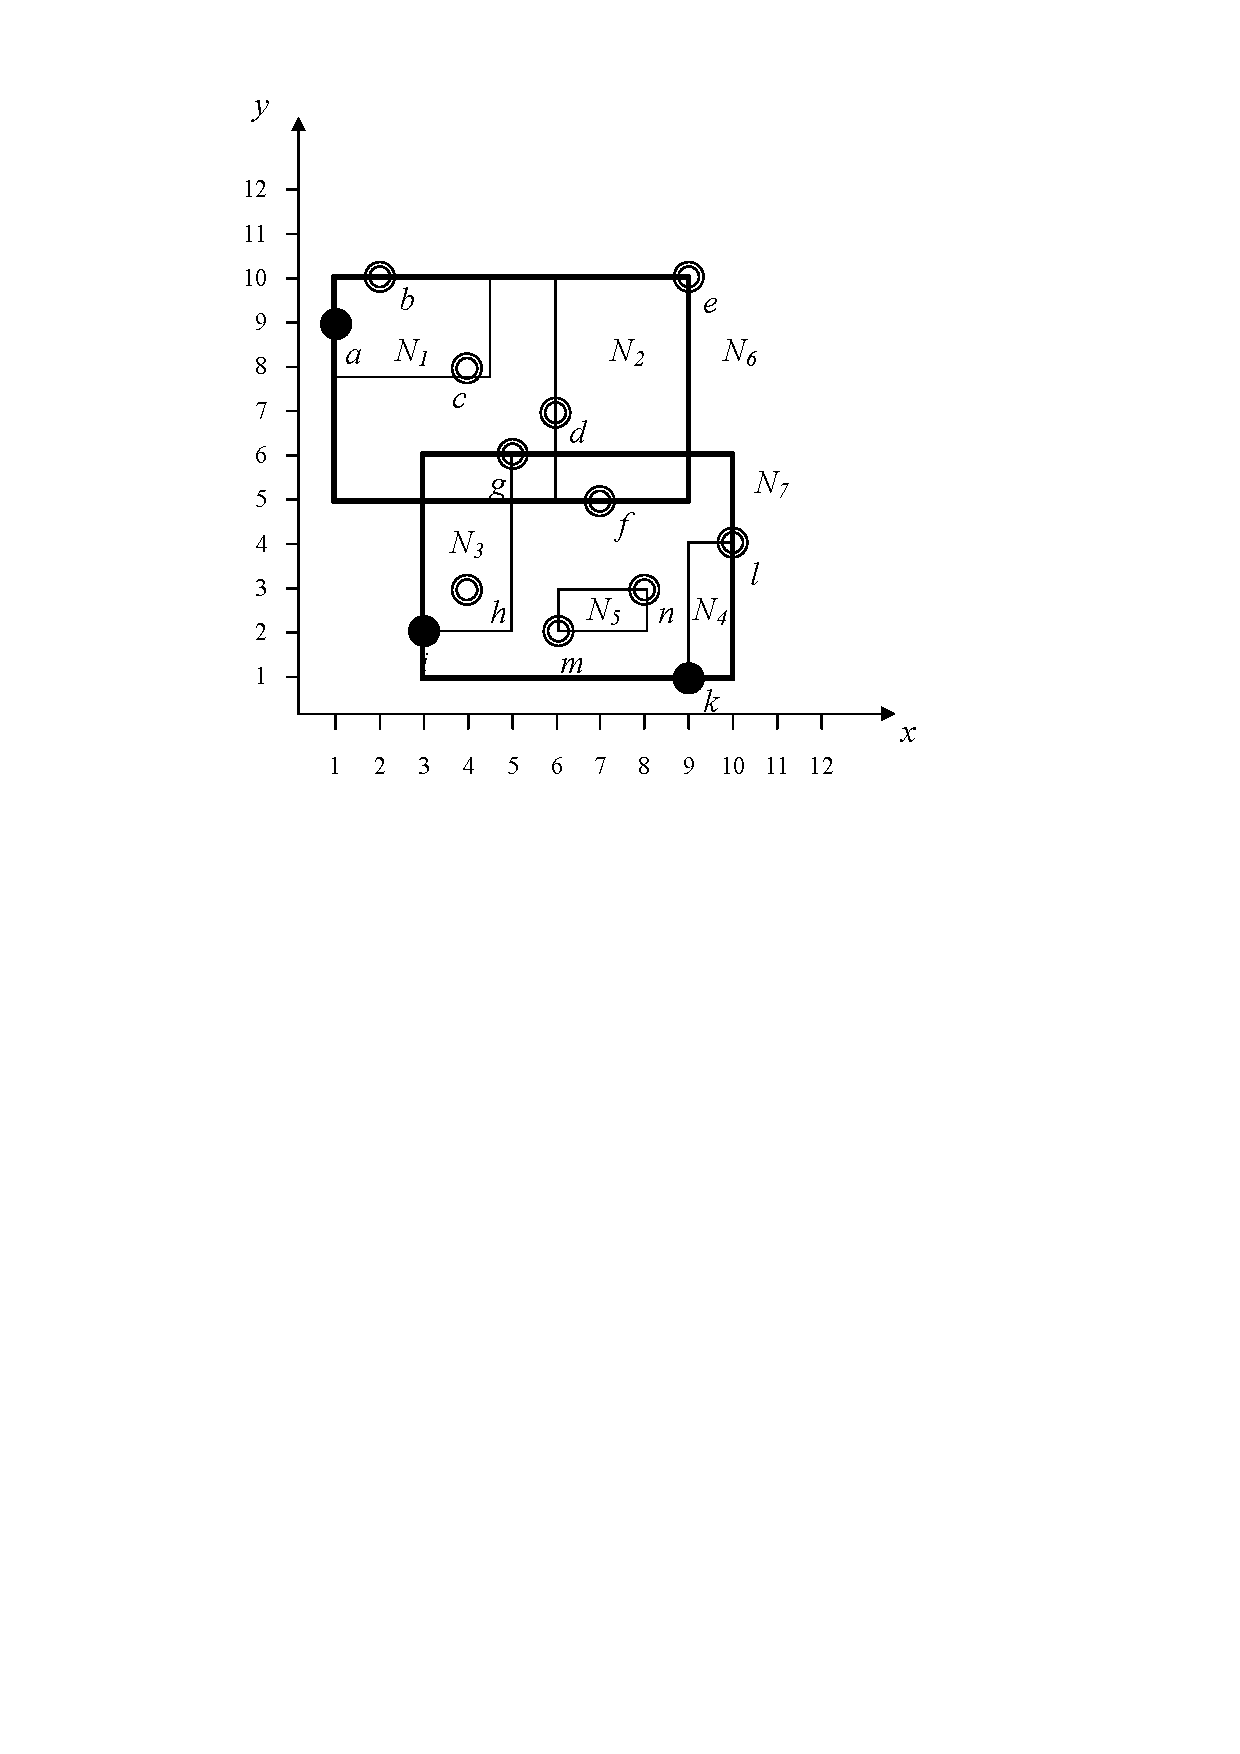
\includegraphics[width=0.35\textwidth]{./FIGs/Fig_SkyRtree1.pdf}
        \label{F:Fig_SkyRtree1} }
    \hspace{0.05in}
        \subfigure[R-tree结构图] {
        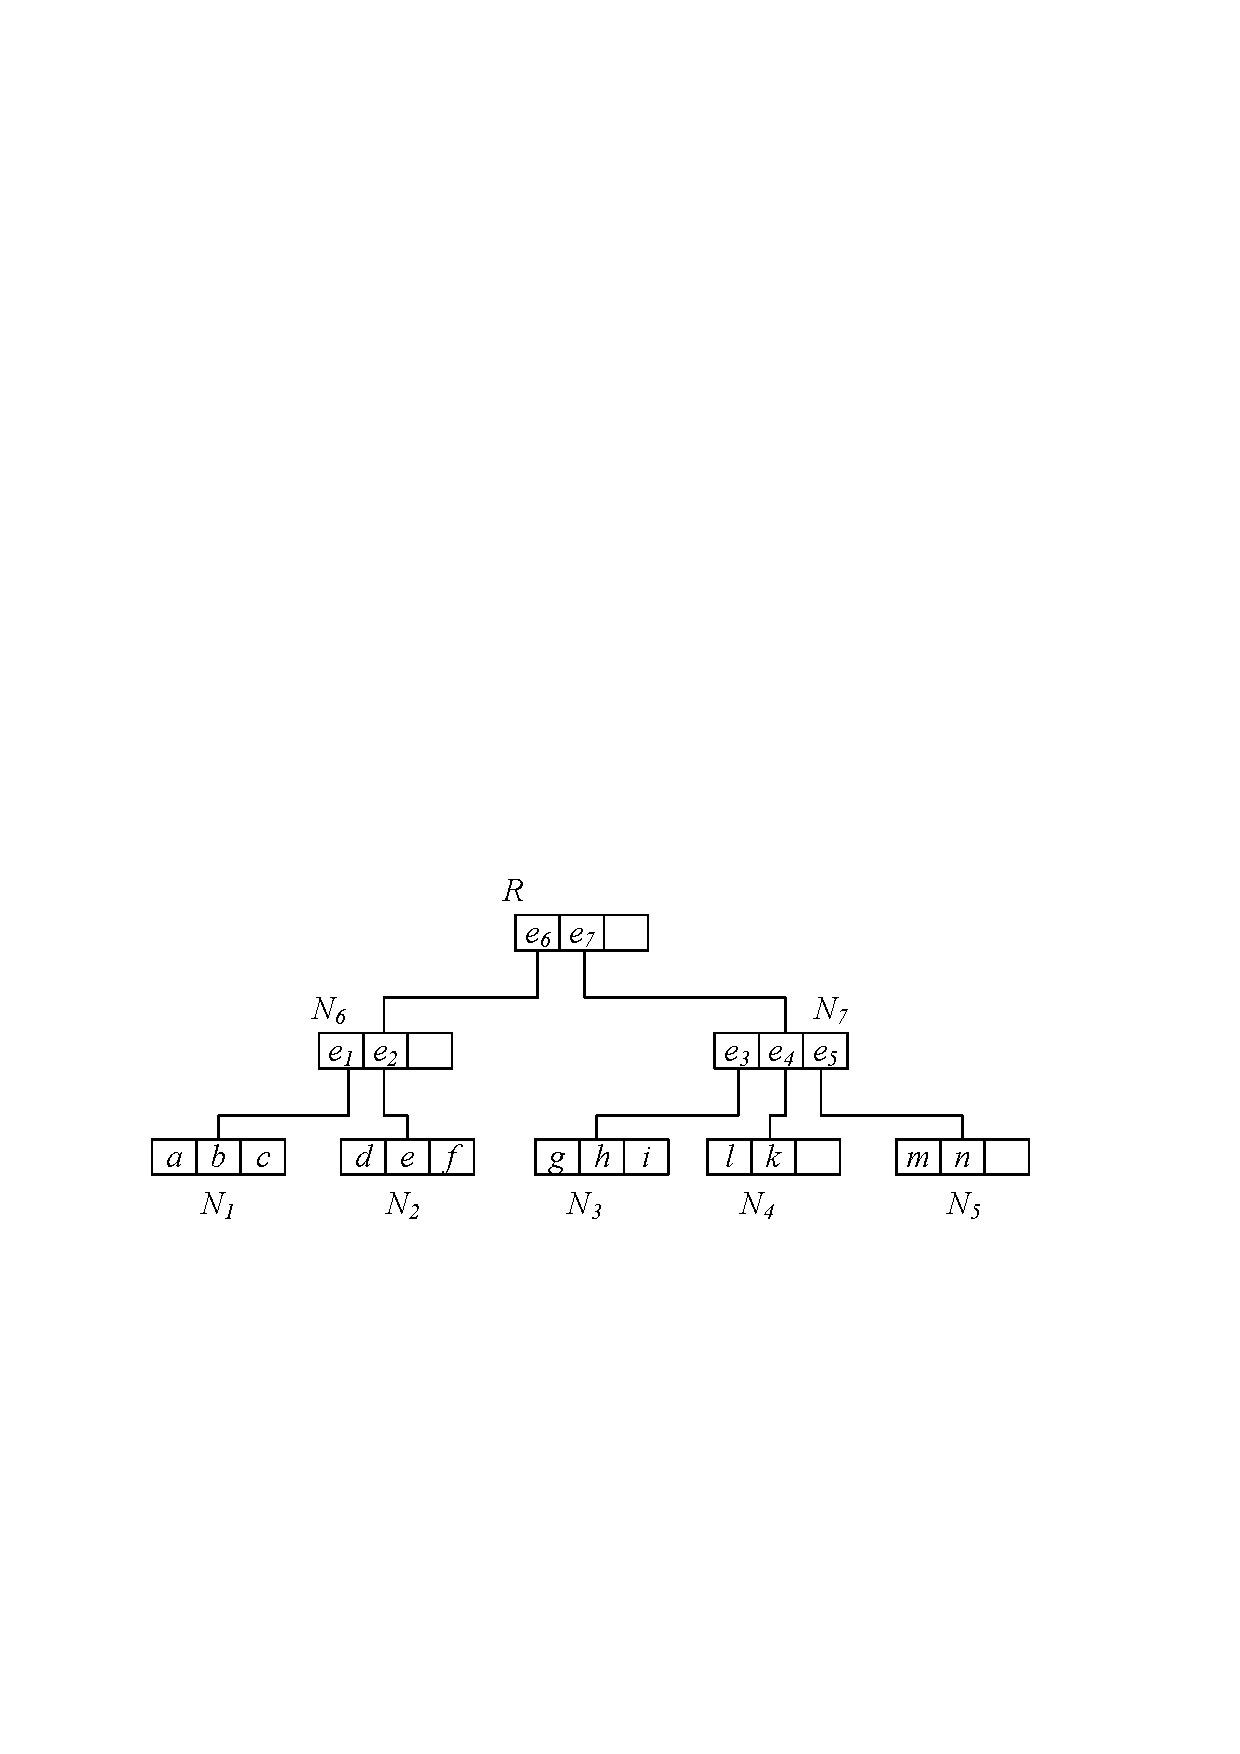
\includegraphics[width=0.55\textwidth]{./FIGs/Fig_SkyRtree2.pdf}
        \label{F:Fig_SkyRtree2}}
    \caption{R-tree例子}
    \label{F:Fig_SkyRtree}
  \end{minipage}%
  \end{figure*}

  该算法也是基于NN算法的策略。算法首先利用R-树结构对数据集中的所有数据建立索引。图~\ref{F:Fig_SkyRtree1}~中所示的是对图~\ref{F:Fig_SkylineHotel}~中的例子建立R-树的索引形成图~\ref{F:Fig_SkyRtree2}~的结构。每个条目$e_{i}$对应下层节点$N_{j}$ 的最小边界矩形(Minimum Bounding Rectangle,~MBR)。叶子节点对应具体的数据对象,规定每个点的最小距离等于它在各个维度属性值的坐标之和,一个MBR 的最小距离为这个矩形左下角数据对象在各个维度上属性值的坐标之和。算法从R-树的根节点出发,将其中所有树中元素根据它们的最小距离有序的插入到一个最小堆中。如果堆不为空,那么取出堆顶元素,如果它不被Skyline集合中的数据对象支配,就对其进行分扩展,将其孩子节点插入到堆中。如果从堆中拿出的是叶子节点,且不被Skyline集合中的数据对象支配,那么就将其插入到Skyline中。

\end{enumerate}

随着数据对象维度的增长,属于Skyline的数据对象会变得越来越大,这会给用户重新带来负担(因为Skyline提出的初衷是减少用户的搜索空间)。为了控制Skyline数据对象集合的大小,有学者对Skyline的基本概念进行扩展。文献~\cite{chan2006finding}~ 中提出了$k$-支配关系的概念,一个数据对象$p$,$k$-支配另一个数据对象$q$,当且仅当$p$ 中存在$k$个属性的值与$q$ 的相应属性一样好,且在这$k$个属性中,至少有一个属性要完全优于$q$。文献~\cite{benouaret2011use}~中基于模糊支配提出了$\alpha$-支配的概念,$\alpha$-Skyline偏向于各个维度属性都很好的数据对象,除此之外,通过改动$\alpha$的值,用户可以灵活的控制Skyline 的大小。在文献~\cite{benouaret2012ws}~中,作者提出了$\sigma$-支配的概念,对于两个互相不支配的数据对象,仍可以计算出它们之间的支配程度,然后从而通过设定$\sigma$值来控制Skyline集合的大小。

\section{组合服务Skyline}

Skyline技术在服务组合领域也被广泛的应用。例如文献~\cite{alrifai2010selecting}~ 中利用Skyline,减少了服务的搜索空间;文献~\cite{zhang2013selecting,tang2012dominance,zhang2013efficient}~ 利用了Skyline 中支配的概念,依据一个组合服务可支配其他组合服务的数量,选出Top-k组合服务;文献~\cite{dai2013using,benouaret2011top}~ 定义了对Skyline中支配的概念做了扩展,分别定义了支配度(或这说支配分值),然后利用该分值对Web服务进行排序。

Qi Yu等人~\cite{yu2013efficient}~提出了组合服务Skyline概念,一个组合服务属于Skyline,当且仅当其不被其他所有的组合服务支配。利用组合服务Skyline,组合服务代理可以快速的响应用户的请求,因为组合服务Skyline中包含了所有可能的``最优''服务。具体来说,组合服务Skyline中的每一个组合服务$CS$,都对应着一些用户偏好的组合(或者说,用户对每个QoS属性指定的权重的集合),如果用户指定这些偏好组合,那么$CS$ 就会被返回给用户。而非Skyline 的组合服务,无论用户指定何种权重,它们都不会被选中。从而组合服务代理不用进行全局搜索计算,而只需要在组合服务Skyline中搜索满足用户约束且QoS 最优的组合服务即可,通常来说会获得较高的效率。本节接下来的部分将简要的介绍~\cite{yu2013efficient}~是如何求解组合服务Skyline的。

首先先来介绍一下~\cite{yu2013efficient}~中相关定义与定理。

\begin{definition}[服务Skyline]
服务Skyline(Service Skyline,~\emph{SSKY})是一个\emph{Web}服务的集合,这个集合中每一个服务$s$,都不被$s$所在的候选服务集合中的其他服务支配。
\end{definition}

\begin{definition}[组合服务Skyline]
组合服务Skyline(Composite Service Skyline,~\emph{CSKY})是一个组合服务的集合,这个集合中的每一个组合服务$CS$,都不被其他组合服务支配。
\end{definition}

\begin{definition}[服务分值]
一个有$d$维QoS属性的服务$s$的分值是$score_{s}=\sum_{i=1}^{d}q_{i}(s)$。
\end{definition}

\begin{property}[]\label{P:Prop_QYuScore}
如果$s_{1} \succ s_{2}$($CS_{1} \succ CS_{2}$),那么$score(s_{1}) < score(s_{2})$($score(CS_{1}) < score(CS_{2}$))。
\end{property}

换句话说,性质~\ref{P:Prop_QYuScore}~说的是,如果服务$s_{1}$的分值比$s_{2}$ 的分值小,那么$s_{2}$一定不可能支配$s_{1}$。

\begin{theorem}[局部搜索策略]\label{TH:Theo_LocalStratey}
给定一个抽象组合服务$\emph{ACS}=\{S_{1}, S_{2}, \cdots, S_{m}\}$ (包含了$m$ 个抽象服务),以及给定每一个抽象服务对应的服务Skyline:$\{\emph{SSKY}_{1}$, $\emph{SSKY}_{2}$, $\cdots$, $\emph{SSKY}_{m}\}$,对应于~\emph{ACS} 的组合服务Skyline,只要在$\{\emph{SSKY}_{1}$, $\emph{SSKY}_{2}$, $\cdots$, $\emph{SSKY}_{m}\}$ 计算即可。
\end{theorem}

在本节接下来的部分,将介绍文献~\cite{yu2013efficient}~中提出三个算法。

\subsection{全遍历算法}

全遍历算法(One Pass Algorithm,~OPA)的输入是$m$ 个已经排序的SSKY,输出是CSKY。OPA算法在执行的时候,需要遍历所有的候选的组合服务,在遍历的过程中存储属于CSKY的组合服务。
在OPA算法开始执行的时候,它先从每一个已有序的SSKY列表中取出第一个服务,然后利用这些服务构造出第一个组合服务$CS_{1}$。 很显然,$CS_{1} \in$ CSKY,这是因为$score(CS_{1})$一定是最小的,所以其他的组合服务不可能支配$CS_{1}$。
由于$CS_{1}$具有最小的分值,它最有可能去支配其他服务。因此,在OPA算法中,$CS_{1}$被存储在CSKY列表的顶部,这样其他被$CS_{1}$支配的组合服务可以被早点发现并移除,减少了比较的次数,提高了效率。
处理完$CS_{1}$后,OPA紧接着开始遍历所有剩下的组合服务。如果一个组合服务$CS_{i}$不被CSKY中的其他组合服务支配,那么就将$CS_{i}$插入CSKY中。如果,OPA 算法将会丢弃$CS_{i}$,然后开始处理$CS_{i+1}$。在将$CS_{i}$ 与CSKY 中的组合服务比较时,如果存在一个$CS_{j}$被$CS_{i}$支配,那么就将$CS_{j}$从CSKY中移除。

OPA算法存在一个突出的缺点:存在~\emph{false positive} Skyline组合服务。\emph{false positive} Skyline组合服务指的是那些曾经被放进CSKY 中但在OPA 执行的过程又被移除的服务。之所以会产生\emph{false positive}的情况,是因为OPA没有对如何遍历组合服务做出规定。\emph{false positive} Skyline组合服务的问题会导致额外的CPU以及内存消耗。

\subsection{双渐进算法}

~\cite{yu2013efficient}~中提到,双渐进算法(Dual Progressive Algorithm,~DPA)中所谓的双渐进指的是:渐进的依据组合分值来遍历;渐进的输出Skyline 组合服务。

\subsubsection{基本的渐进遍历(Basic Progressive Enumeration,~BPE)}

与OPA算法类似,DPA的输入依然是所有抽象服务对应的有序的SSKY。利用Lattice 数据结构可以系统的遍历所有的组合服务。图~\ref{F:Fig_Lattice}~ 中展示了基于三个服务Skyline集合$A(a_{1}, a_{2}, a_{3})$、$B(b_{1}, b_{2}, b_{3})$ 以及$C(c_{1}, c_{2}, c_{3})$构造的Lattice结构。

\begin{figure}[thb]
\centering
    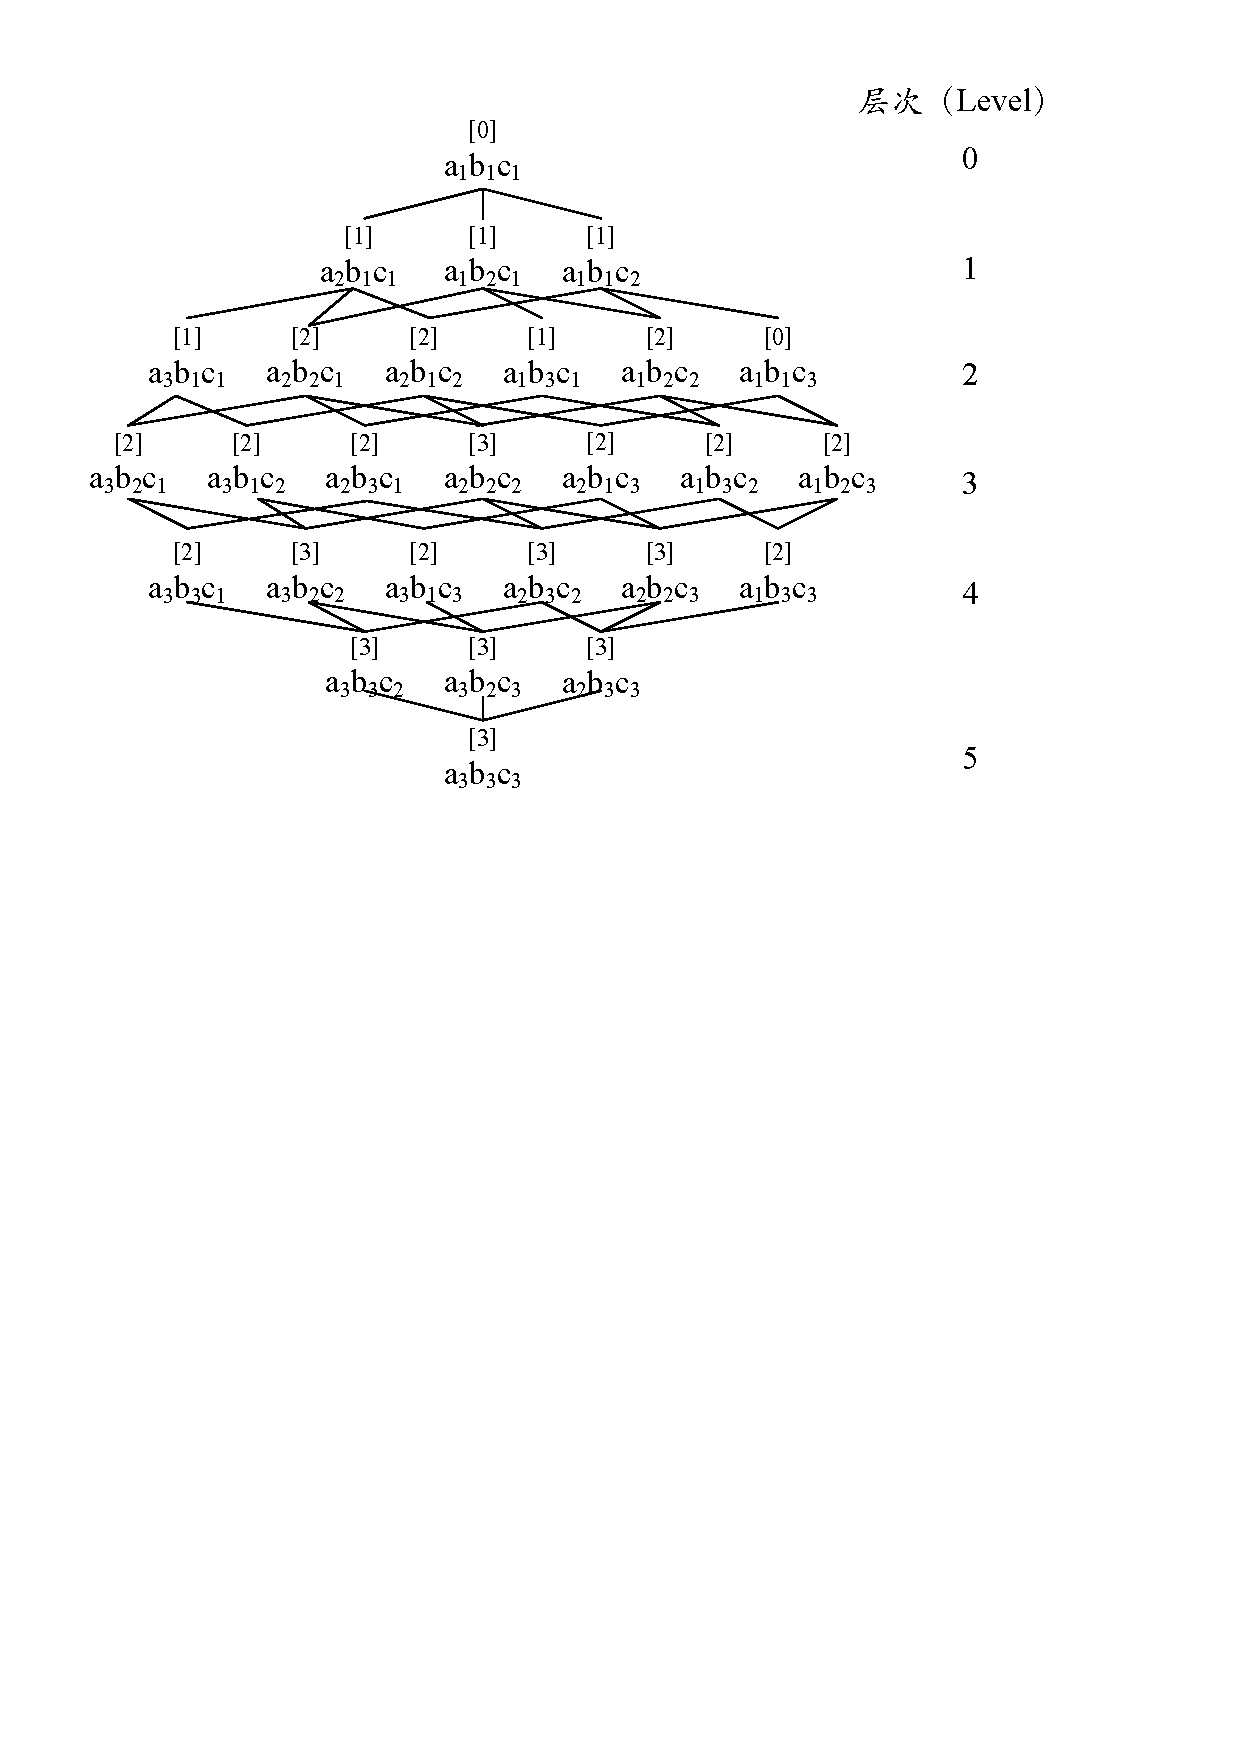
\includegraphics[width=0.8\textwidth]{./FIGs/Fig_Lattice.pdf}
\caption{基于$A(a_{1}, a_{2}, a_{3})$、$B(b_{1}, b_{2}, b_{3})$以及$C(c_{1}, c_{2}, c_{3})$构造的Lattice结构}
\label{F:Fig_Lattice}
\end{figure}

由这三个服务Skyline生成的组合服务数量一共是$|A|\times|B|\times|C|=27$ 个。Lattice中的每一个节点都对应着一个组合服务。Lattice的根节点对应着$CS_{1}$。 孩子节点与父节点中只有一个原子服务不同,在子节点中的这个与父节点不同的原子服务是父节点中相应原子服务的后续原子服务。在Lattice 中,子节点的分值比祖先节点的分值要大。因此,Lattice保证了一个子节点一定在其祖先节点被访问后自身才会被访问到。除此之外,对于一个节点和其祖先的兄弟节点,我们需要进一步判断,来确定访问的顺序,例如:第2层的$score((a_{1},b_{3},c_{1}))$可能比第1层的$score((a_{2},b_{1},c_{1}))$ 要小,因此$(a_{1},b_{3},c_{1})$应该被更早的访问。

为了解决这个问题,文章的作者提出结合使用Lattice 结构$L$和堆结构$H$来确定组合服务的访问的顺序。Lattice可以保证,一个节点一定比其子节点先被访问。堆结构,保证了没有直接血缘关系的节点之间的访问顺序。初始$H$中为$CS_{1}$。当$H$不为空时:(\emph{抽取})先从$H$ 中取出分值最小的组合服务,然后与CSKY中的组合服务进行比较,如果其被支配则丢弃该组合服务,否则将该组合服务插入CSKY;(\emph{扩展})在插入完成后,将其子节点插入到$H$ 中。当$H$ 为空的时候,算法结束。

\subsubsection{父表(Parent Table)}

BPE中存在的一个主要问题是,一个节点可能会被扩展多次。当一个抽象组合服务包含了$m$个抽象服务,那么Lattice中的一个节点最多可有$m$个父节点,故而同一个节点其每一个父节点\emph{抽取}后,将被多次\emph{扩展}。图~\ref{F:Fig_Lattice}~中每个节点顶部的数字代表着其父节点的数量。例如:$(a_{2},b_{2},c_{2})$将会被插入$H$中3 次,因为其有3个父节点。节点被重复的扩展会不仅导致程序产生过量的计算,更严重的是,它有可能会被多次插入到CSKY中,导致结果出错。

为了解决这个问题,作者引入了一个新的数据结构\emph{父表},\emph{父表}以相对较小的代价解决了节点被重复\emph{扩展}的问题。父表存储了与一个给定节点相关的父节点的信息。需要遵守的基础性原则是:\emph{一个节点被插入到$H$,当且仅当其父节点都已被处理了}。首先,我们先来看看如何确定一个节点父节点的数量。基于Lattice,我们可以有如下发现。

\begin{property}[]\label{P:Prop_QYuParentCount}
假设~\emph{SSKY}~中的原子服务的下标是从~\emph{1}~开始。那么对于~\emph{Lattice}~中的某个节点$n_{i}=(s_{1i},s_{2i},\cdots,s_{mi})$,那么$n_{i}$父节点的数量为组成其的原子服务中下标大于1 的服务个数。
\end{property}

利用性质~\ref{P:Prop_QYuParentCount}~,我们可以很容易的得出一个节点的父节点数量,例如,图~\ref{F:Fig_Lattice}~中,$(a_{2},\ b_{2},\ c_{2})$中下标大于~1~的原子服务数量为~3~,因此它的父节点数量为~3~。 利用\emph{父表},遍历的过程可以稍作改进得到一个新的算法(Progressive ENumeration,~PEN)。我们记\emph{父表}为$P$,它先被初始化,每一个节点的父节点个数利用性质~\ref{P:Prop_QYuParentCount}~ 计算得到。与BPE 的实现相似,$H$ 依然是先用$L$ 中的根节点初始化,当$H$不为空的时候:(\emph{抽取})先从$H$ 中取出分值最小的组合服务,然后与CSKY 中的组合服务进行比较,如果其被支配则丢弃该组合服务,否则将该组合服务插入CSKY;(\emph{扩展})在插入完成后,将其子节点取出,然后进行(\emph{更新检查}),\emph{更新检查}是这样做的,当子节点被取出时候,将此子节点在$P$ 中对应的父节点数量减去~1~,并检查此时子节点的父节点数量是否变为~0~,如果为~0~,那么该子节点就可以插入到$H$ 中,否则忽略对此子节点的此次\emph{扩展}。当$H$为空的时候,算法结束。通过这些操作,我们可以确保只有一个子节点的父节点都被处理过了,该子节点才会被插入到堆中。

\subsection{自底向上算法}\label{S:SEC_BUA}

DPA算法的性能由两个因素决定:堆操作以及Skyline比较。当候选服务数量增长的时候,对操作与Skyline比较次数都会指数级的增长。作者提出了自底向上算法(Bottom-Up Algorithm,~BUA),利用了线性组合策略(如图~\ref{F:Fig_LinearComp}~),大大减少了堆操作以及Skyline比较的次数。并且BUA也继承了DPA的所有优点。

\begin{figure}[thb]
\centering
    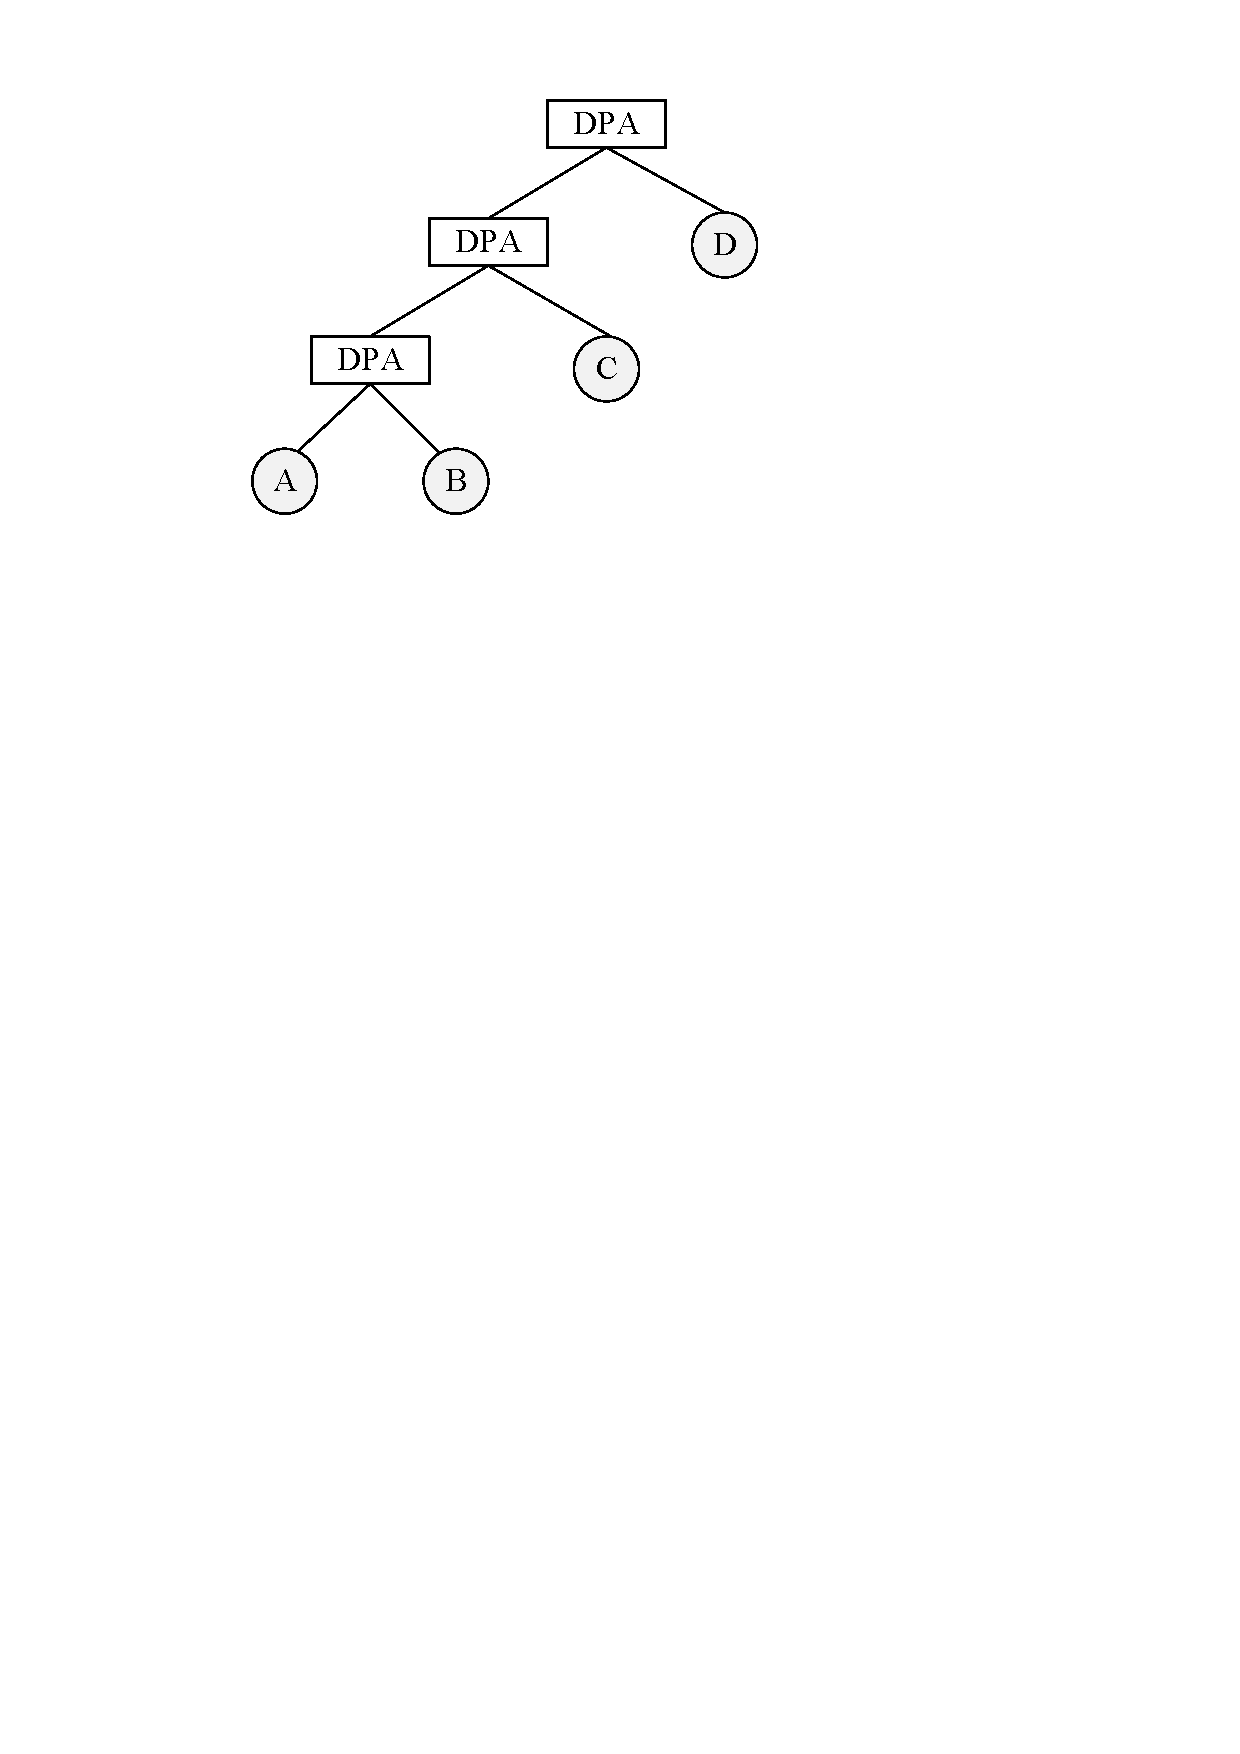
\includegraphics[width=0.5\textwidth]{./FIGs/Fig_LinearComp.pdf}
\caption{线性组合策略}
\label{F:Fig_LinearComp}
\end{figure}

\begin{theorem}[自底向上策略]\label{TH:Theo_BUStrategy}
如果某个组合服务$n_{i}^{m+1}$代表了$(s_{1i},s_{2i},\cdots,s_{(m+1)i})$属于$(m+1)$-\emph{CSKY}(i.e. 基于$(m+1)$个服务计算的Skyline),那么$(s_{1i},s_{2i},\cdots,s_{(m)i})$ 一定属于$(m)$-\emph{CSKY}。
\end{theorem}

定理~\ref{TH:Theo_BUStrategy}~是自底向上策略的理论支撑,该定理表明了如果$n_{i}^{m} \notin$ CSKY,那么$n_{i}^{m}$不可能是任何属于$(m+1)$-CSKY的组合服务的一部分。因此,在计算$(m)$-CSKY的时候,可以放心的将其他非Skyline的组合服务移除。

图~\ref{F:Fig_LinearComp}~中线性组合策略的意思是:如果一个抽象组合服务包含了四个抽象服务,$A$、$B$、$C$以及$D$,先基于$A$与$B$利用DPA计算出2-CSKY,然后基于$A$与$B$的结果再和$C$通过DPA计算出3-CSKY,重复之前的操作,直到与$D$计算,得到最终的CSKY。

\section{支持QoS关联的服务选择}

在现实应用中,可选服务通常不是相互独立的,服务之间可能存在QoS关联。文献~\cite{ye2008service}~中提出了一个支持服务关联关系的QoS描述模型,用于刻画可选服务的QoS对其他可选服务的依赖关系,并给出了一套QoS描述的自动生成方法,并在此基础上提出了支持QoS关联的利服务选择方法,包括基于整数规划求解最优组合服务以及基于启发式求解最优组合服务,但是文中并没有利用支配关系去缩减候选服务的空间。文献~\cite{barakat2012efficient}~ 利用析取范式(DNF)来一个服务中,某个关联值生效的条件,并利用支配的思想对候选服务的空间做削减,最后给出了一个计算QoS 最优组合服务的方法,然而文章中生成关联值生效的条件算法过于复杂。文献~\cite{deng2014service}~中考虑了QoS关联的情况,并提出了一个预处理算法,先在每一个候选集合中移除一部分服务,然后再进行最优QoS组合服务的选择,然而文中的预处理规则并不完善,作者忽略了一个服务可能会影响多个服务QoS值的情况,导致预处理算法在遇到这种情况时会错误的处理,另外作者仅考虑了一维QoS的情况。文献~\cite{zhang2014correlation}~中利用频繁项集的方法去挖掘服务的运行日志,从而找到服务之间的QoS关联关系,然而通过日志来挖掘关联关系的前提是,之前执行过这些有关联的服务,但是在不知道哪些服务有关联的情况下,人们通常会选择默认QoS 值比较优秀的服务,导致有关联的且QoS不是特别好的服务得不到选择,因此日志中根本不会有这些执行信息,作者也没有解释如何处理这类情况。

\section{本章小结}

本章介绍了Web服务与服务组合的基本概念,随后介绍了Skyline的相关概念以及几种常见的集中式算法,接着介绍了组合服务Skyline 的概念,并详细的介绍相关的算法,最后简要的回顾了支持QoS关联的服务选择的相关工作。

